\documentclass[runningheads]{llncs}

%---- Sonderzeichen-------%
%\usepackage {ngerman}
\usepackage[ngerman, english]{babel}
%---- Codierung----%
\usepackage[latin1]{inputenc}	% for Unix and Windows
\usepackage[T1]{fontenc}
\usepackage{graphicx}
\usepackage{url}
\usepackage{llncsdoc}
%----- Mathematischer Zeichenvorrat---%
\usepackage{amsmath}
\usepackage{amssymb}
\usepackage{enumerate}
% fuer die aktuelle Zeit
\usepackage{scrtime}
\usepackage{listings}
\usepackage{subfigure}
\usepackage{hyperref}

\setcounter{tocdepth}{3}
\setcounter{secnumdepth}{3}

\usepackage{lipsum}
\usepackage{graphicx}



\begin{document}

\mainmatter
%TODO Titel �ndern?????
\title{Deployment Strategies in CI/CD Pipelines}
\titlerunning{Deployment Strategies in CI/CD Pipelines}
\author{Niko Benkler }
\authorrunning{Model-driven Software Quality Engineering}
\institute{Supervisor: Dr. Robert Heinrich \\ \href{mailto:robert.heinrich@kit.edu}{robert.heinrich@kit.edu}}
\date{13.01.2018}
\maketitle

\begin{abstract} 
 	In the last decade, software development experienced a huge transition. Since agile methodologies were introduces in the early 2000, software development became faster and faster. Today, another software development process is emerging: Continuous Software Engineering (CSE). CSE, especially Continuous Integration(CI), Continuous Delivery(CDE) and Continuous Deployment(CD) receive more and more attention in organizations such as Facebook, Paddy Power and Atlassian but also in small start-up companies. 
 	It enables them to e.g. deliver software more frequently, reduce time-to-market, obtain customer feedback faster, build the right product or to improve product quality. 
 	Therefore, this seminar paper presents the current state of the art concerning Continuous Practices, compares the traditional deployment strategies with the new CSE practices and proposes some tools, that can be used in a CI/CD Pipeline to support CSE. 
 	% TODO: da fehlt noch was 10 scientific paper and a book were studied, in order to cover 
 	\\
 	\\
 	\textbf{Keywords - }Agile, continuous software development, continuous integration, continuous delivery, continuous deployment, DevOps, CI/CD Pipeline
 	 
	

\end{abstract}

\tableofcontents
\clearpage


\section{Introduction}
Today, the software development process has to face many difficult demands. Fast-changing and unpredictable markets, changing customer requirements \cite{claps2015journey} and rapidly advancing information technologies \cite{olsson2012climbing} require a faster process of software development. 
To achieve this, several organizations adopt Continuous Practices in order to extend their agile practices \cite{claps2015journey}. Therefore, releasing software becomes even faster. 
\\
This seminar paper presents an evolution path, called 'stairway to heaven' \cite{olsson2012climbing}, which describes a possible transition from traditional development towards CD. 
As the core of CDE is a deployment pipeline \cite{schermann2016empirical}, the paper also presents its usual phases and the possible tools, that support each phase.
Nevertheless, studying several papers revealed, that CDE not only comes with benefits, but also with huge social and technical challenges \cite{claps2015journey}. The paper clarifies them and proposes some mitigation strategies. 
%TODO  Stimmt der remainder noch???
The remainder of the seminar paper is structured as follows: In section II, we define the terminology. Section III describes a possible transition from traditional deployment to CD based on the 'stairway to heaven' model \cite{olsson2012climbing}. That section is followed by the explanation of a possible pipeline and the available tools which can be used to support the tasks of each phase.  Section V discusses the challenges that is caused by CDE and possible mitigation strategies. Finally, I present my conclusion in section VI.

\section{Background}
Here, I give an overview of the most important keywords. Those keywords are necessary to understand the content of the seminar paper. When studying the given information about Continuous Software Engineering (CSE), one could clearly see that there are no universally accepted definitions \cite{schermann2016empirical}. Therefore, the following subsections provide the definitions as they are used in this seminar paper.

\subsection{Agile Methodologies}
Agile software development is based on "iterative development, where requirements and solutions evolve through collaboration between self-organizing cross-functional teams" \cite{taheritanjani2016comparison}. It encourages adaptive planning, early delivery and continuous improvement.
Besides, other characteristics such as flexibility, efficiency, speed, the ability to react to fast changing customer requirements and fluctuating market needs \cite{olsson2012climbing} make agile methodologies so attractive for organizations. 
As mentioned before, agile methodologies were introduced in the early 2000 \cite{shahin2017continuous}. So far, many development companies succeeded in implementing agile methodologies.
However, agile software development 'only' allows frequent software releases but no continuous releases. The difference becomes clear, when it comes to the comparison of traditional deployment and CD.  

\subsection{DevOps}
 "DevOps is a set of practices intended to reduce the time between committing a change to a system and the change being placed into normal production, while ensuring high quality" \cite{bass2015devops}. It is a coined word, that stands for Development (Dev) and Operations (Ops). The main task is bringing together programmers, testers and quality insurance engineers but also  IT operations staff \cite{claps2015journey} to shorten feedback loop. According to \cite{bass2015devops}, the DevOps practices can be differentiated in 5 categories:
 \begin{itemize}
 	\item Treat Ops as "first-class citizens". This means, the involvement of operations in the development process. 
 	\item Dev has to be more responsible for incident handling to shorten the time between error observation an the error fix.
 	\item Include both, Dev and Ops into the deployment process in order to avoid errors caused by buggy deployment.
 	\item Use continuous deployment.
 	\item Use deployment scripts and other infrastructure code. This code is subjected to the same quality control practices than the application code. As a result, deployment error due to misconfiguration can be mitigated.
\end{itemize}

\noindent Especially the fourth category shows the close connection between DevOps practices and continuous practices.

\subsection{Continuous software engineering}
Continuous software engineering (CES) is a practice that promotes the development, deployment and the release of software products in very short cycles, typically hours or days. \cite{shahin2017continuous} \cite{taheritanjani2016comparison}. As a direct consequence, quick feedback allows i.a.: to determine new functionality to build, feature prioritization, information about the suitability of the current software architecture, to gather data for decision making in general. CES requires agile methodologies and DevOps practices \cite{taheritanjani2016comparison}. According to \cite{shahin2017continuous}, CES involves 3 phases: Business Strategy and Planning, Development, Operations. This seminar paper focuses on the three development activities: continuous integration, continuous delivery and continuous deployment. Fig. \ref{Fig RelCSE} demonstrates the relationship between CI, CDE and CD.

\subsubsection{Continuous Integration}
Continuous Integration (CI) is a CSE practice, in which developers integrate and merge their work into a shared repository very frequently, for example multiple times a day \cite{shahin2017continuous} \cite{schermann2016empirical}. Also,  automated builds and test permit to discover integration errors as fast as possible. CI improves  the effectiveness of a team as much as the software quality \cite{shahin2017continuous}. In other words, CI ensures, that the software is always in a ready to deploy state \cite{claps2015journey}.
\subsubsection{Continuous Delivery}

\subsubsection{Continuous Deployment}

\begin{figure}[h]
	\centering
	\resizebox*{1.0 \textwidth}{!}{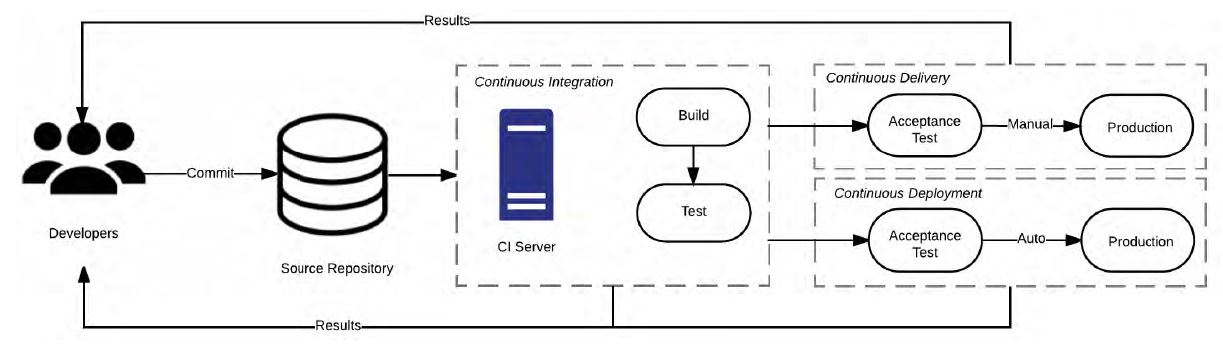
\includegraphics
		{RelCSE}}  
	\caption{\label{RelCSE}The relationship between CI, CDE, CD \cite{shahin2017continuous}} 
\end{figure}



\bibliographystyle{itmalpha}
% TODO: �ndern der folgenden Zeile, damit die .bib-Datei gefunden wird
\bibliography{literatur}

\end{document}

